\chapter{Cum sunt extrase reperele faciale}
\label{chapter6}
Utilizând cu succes reperele faciale pentru a localiza și a extrage ochii, ca apoi să folosesc aceste date pentru o rețea convoluțională ca să urmăresc ochii utilizatorului, am devenit interesat de cum funcționează biblioteca Python pe care am folosit-o (dlib) pentru a găsi aceste repere faciale.
Am decis să studiez puțin această problemă și, conform \cite{paper_stacked_hourglass}, metoda ``state-of-the-art'', de ultimă oră, pentru detectarea reperelor faciale se bazează pe arhitectura de tipul \emph{Hourglass} care este, într-o formă simplă a ei, o arhitectură de tipul \emph{Autoencoder} (Encoder-Decoder).

\begin{figure}[h]
    \centering
    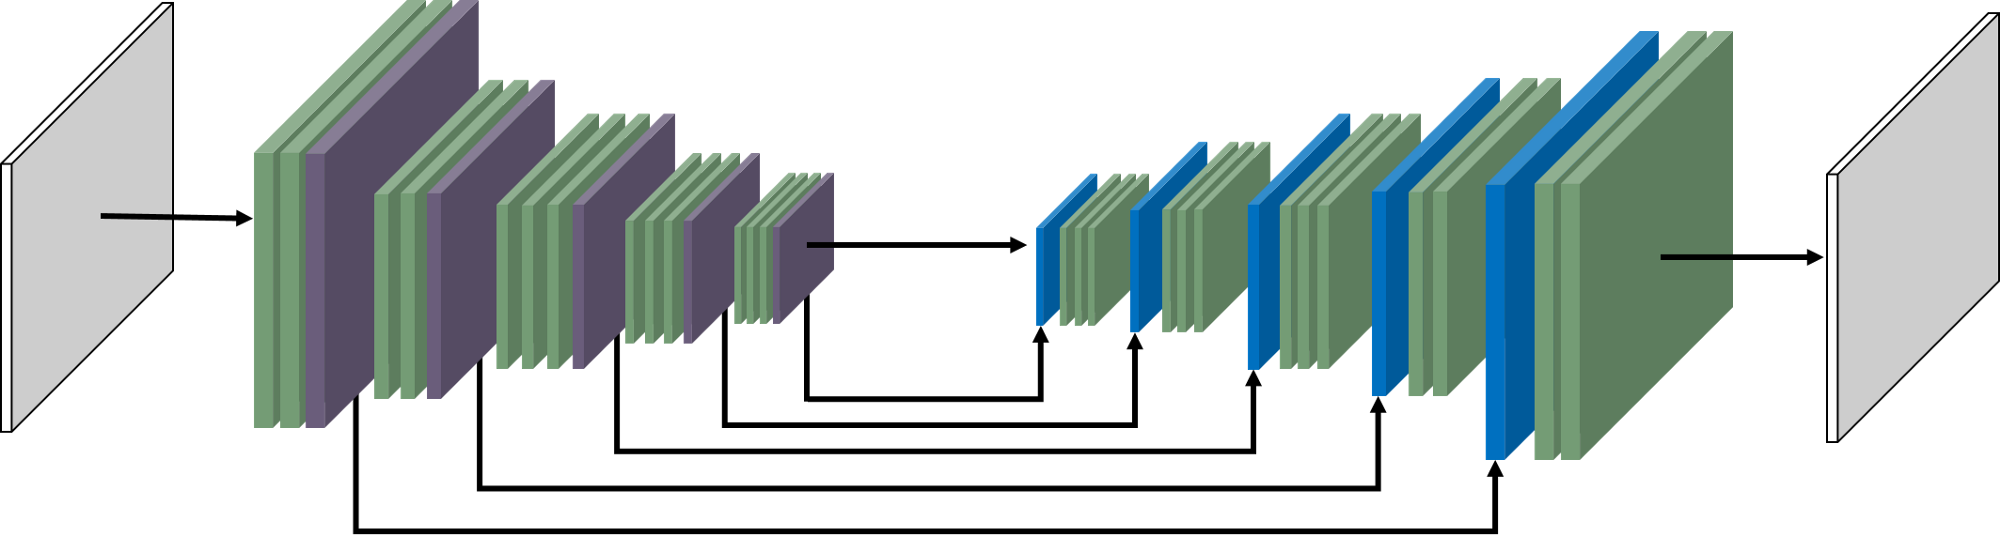
\includegraphics[width=\textwidth]{hourglass.png}
    \caption{Exemplu de arhitectură Hourglass}
\end{figure}

M-am concentrat doar pe prezicerea centrului unui ochi, plecând de la o mulțime de date care conține imagini ale ochiului.
Ca date de antrenament am folosit mulțimea de date pusă la dispoziție pusă la dispoziție de \emph{crowdpupil}\footnote{\url{http://cs.uef.fi/pupoint/}}, care constă în 792 de imagini, fiecare imagine fiind etichetată cu poziția centrului ochiului în acea imagine.

Din căutările pe care le-am efectuat, am descoperit că există două metode de a încerca prezicerea reperelor faciale.
Prima metoda se ocupă cu găsirea coordonatelor exacte $(x, y)$ a fiecărui reper facial prin regresie, iar a doua metodă încearcă construirea unor hărți termografice (\emph{heatmaps}) care codifică acele repere faciale.

Am ales cea de-a doua opțiune, așa că am generat, pentru fiecare imagine a ochiului din mulțimea de date crowdpupil, o hartă termografică care codifică centrul ochiului.
Acest lucru l-am făcut prin a construi o \emph{Distribuție Gaussiană} multivariată (2D), definită prin
$$\mathcal{N}(\mu, \Sigma) = \frac{1}{\sqrt{(2\pi)^{n}|\Sigma|}}exp(-\frac{1}{2}(X-\mu)^T\Sigma^{-1}(X-\mu))$$

În cazul de față am definit $\mu$ și $\Sigma$ astfel:
$$\mu = (x, y), (x, y)$$
$$\Sigma = (f(r), f(r))$$
$\mu$ fiind coordonatele centrului ochiului iar $r$ raza pupilei.

Am calculat o medie pentru valoarea lui $r$ uitându-mă la o parte din imagini iar apoi am definit $f(r) = 1.5 * r$.
Având acestea definite, am putut codifica centrul ochiului fiecărei imagini:

\begin{figure}[h]
    \centering
    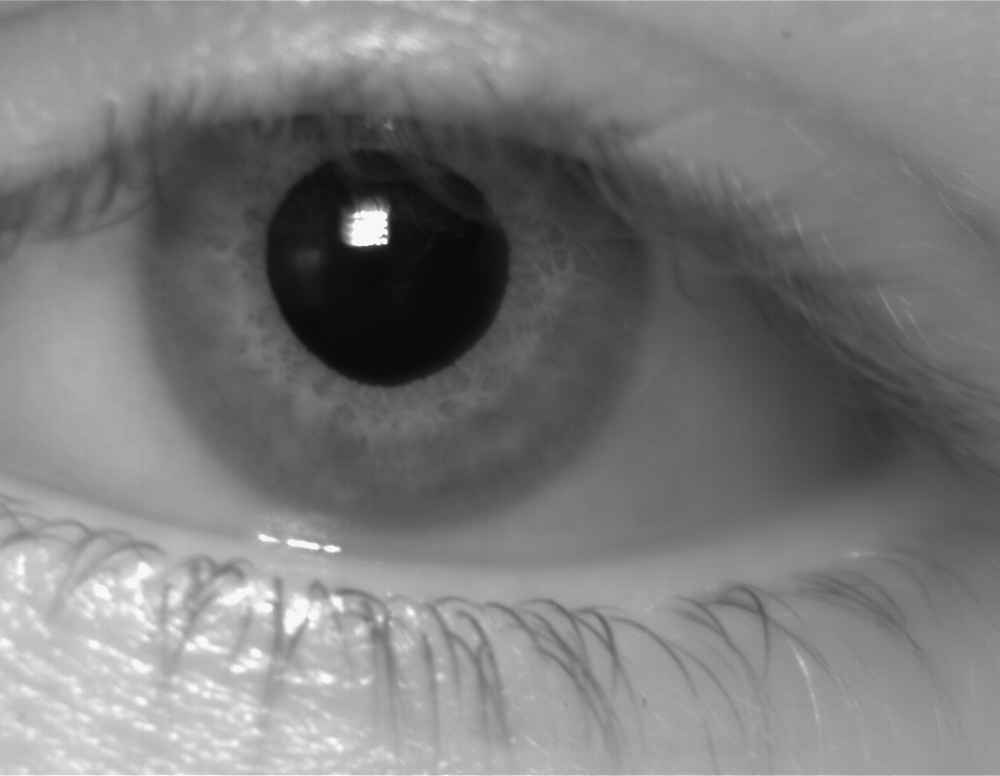
\includegraphics[width=0.32\textwidth]{Img_002_L_2.jpg}
    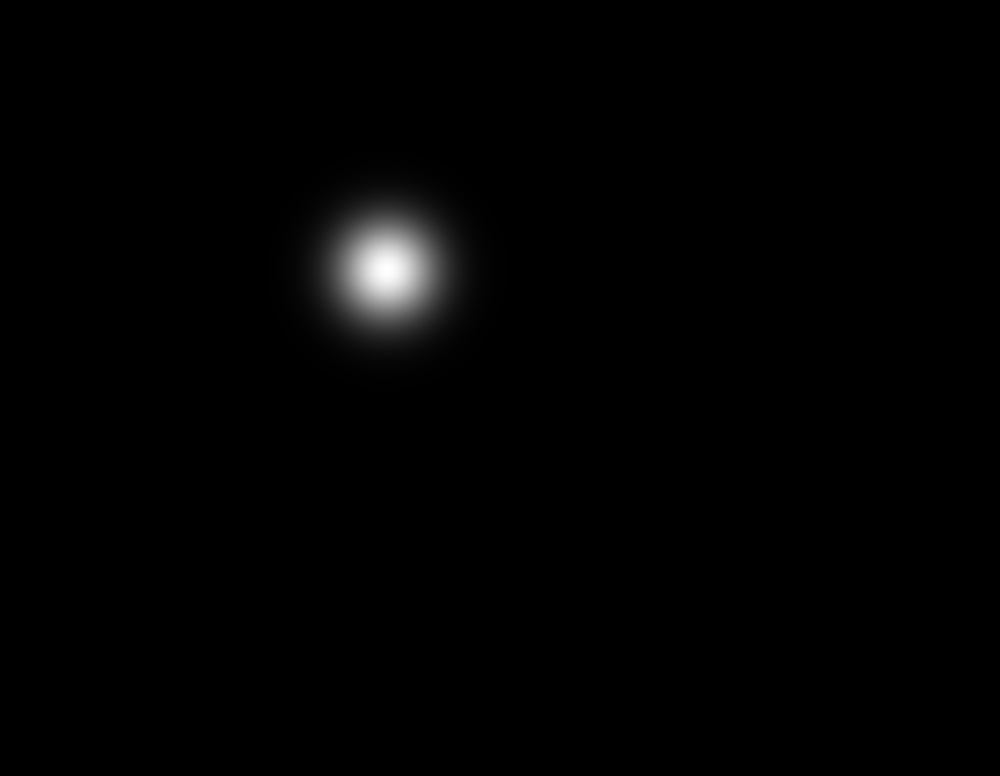
\includegraphics[width=0.32\textwidth]{h_Img_002_L_2.jpg}
    \caption{Centrul ochiului codificat printr-o hartă termografică}
\end{figure}

Am folosit o formă simplă a arhitecturii Hourglass pentru a încerca reconstruirea acestei hărți termografice.
Arhitectura se bazează pe 2 părți corespunzătoare unei arhitecturi \emph{Encoder–Decoder}.
Prima parte produce o \emph{compresie} a informației, iar a doua parte o \emph{decompresie} pentru a încerca reconstruirea imaginii inițiale.
În acest fel, rețeaua învață să folosească doar acele informații care sunt de folos din imaginea originală și care aduc un plus de informație pentru rezultatul final.
Iată arhitectura pe care am folosit-o:

\begin{lstlisting}[language=python]
class MyCNN(nn.Module):
    def __init__(self, input_size):
        super(MyCNN, self).__init__()
        ## eye image -> encoder -> decoder -> heatmap
        filters = [16, 32, 64, 128]
        # starting encoding
        self.layer1 = nn.Sequential(
            nn.Conv2d(1, filters[0], kernel_size=3, padding=2),
            nn.MaxPool2d(kernel_size=2, stride=2, padding=1),
            nn.ReLU(inplace=True),
            nn.BatchNorm2d(filters[0]),
            
            nn.Conv2d(filters[0], filters[1], kernel_size=2, padding=2),
            nn.MaxPool2d(kernel_size=2, stride=2, padding=1),
            nn.ReLU(inplace=True),
            nn.BatchNorm2d(filters[1]),
            
            nn.Conv2d(filters[1], filters[2], kernel_size=3, padding=2),
            nn.MaxPool2d(kernel_size=2, stride=2, padding=1),
            nn.ReLU(inplace=True),
            nn.BatchNorm2d(filters[2]),
            
            nn.Conv2d(filters[2], filters[3], kernel_size=2, padding=1),
            nn.MaxPool2d(kernel_size=2, stride=2, padding=1),
            nn.ReLU(inplace=True),
            nn.BatchNorm2d(filters[3]),
        )
        # encoding done, starting decoding
        self.layer2 = nn.Sequential(
            nn.Upsample(size=(28, 35), mode='bilinear'),
            nn.ConvTranspose2d(filters[3], filters[2], kernel_size=2, stride=1, padding=1),
            nn.ReLU(inplace=True),
            nn.BatchNorm2d(filters[2]),
            
            nn.Upsample(size=(54, 68), mode='bilinear'),
            nn.ConvTranspose2d(filters[2], filters[1], kernel_size=3, stride=1, padding=2),
            nn.ReLU(inplace=True),
            nn.BatchNorm2d(filters[1]),
            
            nn.Upsample(size=(104, 132), mode='bilinear'),
            nn.ConvTranspose2d(filters[1], filters[0], kernel_size=2, stride=1, padding=2),
            nn.ReLU(inplace=True),
            nn.BatchNorm2d(filters[0]),
        
            nn.Upsample(size=(202, 258), mode='bilinear'),
            nn.ConvTranspose2d(filters[0], 1, kernel_size=3, stride=1, padding=2),
            nn.ReLU(inplace=True),
            nn.BatchNorm2d(1),
        )
\end{lstlisting}

Partea de compresie corespunde operației de convoluție care reduce dimensiunea imaginii de la un strat la altul în funcție de parametrii convoluției – spre exemplu pasul (saltul) pe care îl realizează filtrul de convoluție.
În partea de decompresie am folosit operația de \emph{Upsampling} care merge înapoi pe pașii convoluției și mărește dimensiunea imaginii, aducându-o la dimensiunea originală (în acest caz imaginile au fost redimensionate la 200x256 pixeli).

Pentru a calcula exact dimensiunea imaginii rezultată ($W_o$ și $H_o$) după o operație de convoluție am folosit următoarele formule:
$$W_o = \frac{W - F_w + 2P}{S_w} + 1$$
$$H_o = \frac{H - F_h + 2P}{S_h} + 1$$
unde $(W, H)$ este dimensiunea înainte de operația de convoluție, $(F_w, F_h)$ este dimensiunea filtrului de convoluție, $P$ este \emph{padding-ul} adăugat imaginii iar $(S_w, S_h)$ dimensiunea pasului pe care îl realizează filtrul de convoluție.

Am antrenat rețeaua pentru 12 epoci, folosind optimizatorul \emph{Adam}, iar eroarea a fost calculată folosind \emph{MSE}.
Pentru ultima epocă, media scorului MSE pentru toate datele de test (în jur de 20\% din datele totale) a fost de $8,425983$.

\begin{figure}[H]
    \centering
    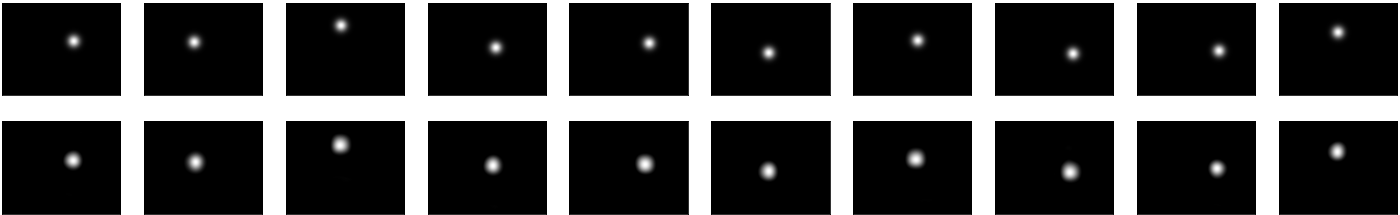
\includegraphics[width=\textwidth]{heatmap_predictions.png}
    \caption{Reconstruirea hărților termografice. Prima linie reprezintă adevărul de bază, iar a doua linie rezultatele modelului antrenat}
\end{figure}

Deși rețeaua a reușit să reconstruiască bine hărțile termografice de mai sus, folosind imagini cu mine în condiții reale nu a dat rezultate bune.
Unul dintre motive ar fi rezoluția webcam-ului care nu este foarte bună și imaginile ochilor extrași sunt de o calitate inferioară.
Este interesant de observat în figura de mai jos că rețeaua a putut identifica aproximativ centrul ochiului pe o imagine care conținea fața mea întreagă, deși nu a fost antrenată în acest sens.

\begin{figure}[h]
    \centering
    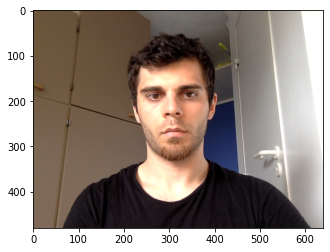
\includegraphics[width=0.32\textwidth]{heatmap_test.png}
    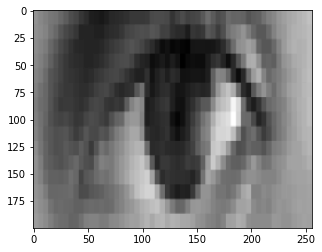
\includegraphics[width=0.32\textwidth]{heatmap_eye.png}
    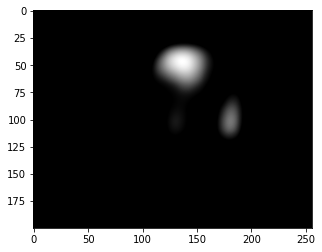
\includegraphics[width=0.32\textwidth]{heatmap_result.png}
    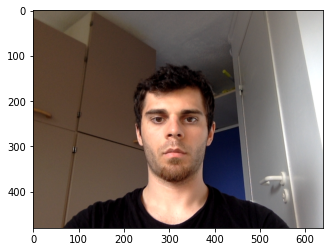
\includegraphics[width=0.32\textwidth]{heatmap_original_2.png}
    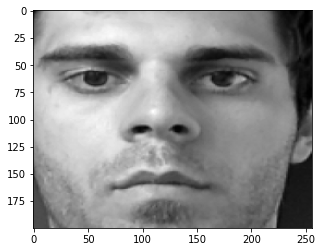
\includegraphics[width=0.32\textwidth]{heatmap_extracted_2.png}
    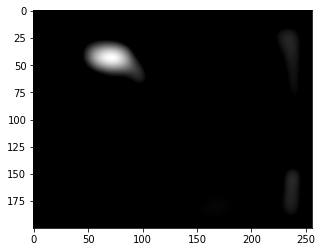
\includegraphics[width=0.32\textwidth]{heatmap_result_2.png}
    \caption{Testarea rețelei de tip Hourglass pe imagini cu mine însumi}
\end{figure}

Acest experiment a servit pentru înțelegerea funcționalității bibliotecilor precum dlib.
Experimentul pe care l-am efectuat a fost unul foarte simplu care poate fi extins la a prezice câte o hartă termografică pentru fiecare reper facial (uzual sunt 68) și la a folosi o arhitectură de tip Hourglass mai avansată, care ar folosi, de exemplu, legături reziduale între straturile de convoluție.
Chiar dacă rezultatele finale nu au fost reușite, experimentul m-a ajutat la înțelegerea metodelor \emph{state of the art} pentru identificarea reperelor faciale.